\documentclass[12pt,a4paper,twocolumn]{article}
\usepackage[utf8]{inputenc}
\usepackage[T1]{fontenc}
\usepackage{polski}
\usepackage[polish]{babel}
\usepackage{geometry}
\geometry{margin=2.5cm}
\usepackage{graphicx}
\usepackage{tabularx}
\usepackage{booktabs} 
\usepackage{hyperref}
\usepackage{bookmark}
\usepackage{enumitem}
\usepackage{titlesec}
\usepackage{microtype}
\usepackage{varwidth}

\title{
    \begin{center}
    
\includegraphics[width=\textwidth]{fig/logo.png}
    \vspace{0.25cm}
    \end{center}
    \textbf{\huge Struktury danych} \\
    \vspace{0.5cm}
    \textit{Analiza porównawcza wydajności list wiązanych i tablic dynamicznych w języku C++}
    }
\author{Piotr Frąc}
\date{Marzec 2026}


\begin{document}
\maketitle
\clearpage
\section{Wprowadzenie}
Projekt skupia się na analizie porównawczej dwóch fundamentalnych struktur liniowych:
\textit{linked list} i \textit{dynamic array} \\ 
Celem pracy jest implementacja obu struktur w języku C++ 
oraz przeprowadzenie testów wydajnościowych dla podstawowych operacji, takich jak:

\begin{itemize}[nosep]
\item dodawanie i usuwanie elementów (na początku, na końcu oraz na zadanym indeksie),
\item wyszukiwanie elementów o określonej wartości,
\item dostęp do elementu poprzez indeks. 
\end{itemize}

Badanie ma na celu wykazanie różnic w złożoności obliczeniowej oraz praktycznym czasie wykonania, 
wynikających ze specyfiki alokacji pamięci
Pełny kod źródłowy projektu wraz z historią zmian dostępny jest w repozytorium pod adresem: 
\url{https://github.com/Elrior-programmer/Struktury-Danych/tree/main/P1%20-%20Lista_wizana} 
\subsection{Zaimplementowane struktury danych}
Wszystkie struktury danych zostały wykonane zgodnie z wykładami i prezentacjami dr inż. Radosława Rudego, które są dostępne pod linkiem: 
\url{https://kam.pwr.edu.pl/jaroslaw-rudy/#tab-struktury-danych-wyklad}
\subsubsection*{Lista wiązana}
\begin{center}
    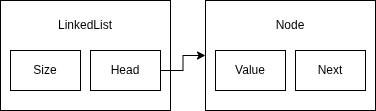
\includegraphics[width=\linewidth]{fig/LinkedList.png}
\end{center}
Zaimplementowana \textbf{lista} jest przykładem \textit{Listy jednokierunkowej liniowej (Singly Linked List)}, 
która charakteryzuje sie:
\begin{itemize}[nosep]
\item \textbf{Jednokierunkowość:} Każdy węzeł (\textit{node})
 przechowuje wskaźnik wyłącznie do swojego następcy. 
 Oznacza to, że przeglądanie struktury możliwe jest tylko od głowy (\textit{head})
w stronę końca listy.

\item \textbf{Liniowość (brak cyliczności):} 
Struktura posiada wyraźnie zdefiniowany początek oraz koniec.
Ostatni element przechowuje wartość pustą (\texttt{nullptr}),
co stanowi jednoznacznie zakończenie sekwencji danych.
\end{itemize}

\subsubsection*{Tablca Dynamiczna}
\begin{center}
    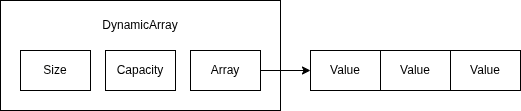
\includegraphics[width=\linewidth]{fig/DynamicArray.png}
\end{center}
Zaimplementowana \textbf{tablica dynamiczna} charakteryzuje się specyficznymi usprawnieniami implementacyjnymi:
\begin{itemize}[label=\textbullet, nosep]
    \item \textbf{Inicjalizacja niezerowa:} Tablica rozpoczyna pracę z domyślną pojemnością $capacity = 4$,
     co eliminuje potrzebę realokacji przy pierwszych operacjach dodawania.
    \item \textbf{Progresja geometryczna ($2 \times capacity$):} 
    W przypadku przepełnienia bufora, jego rozmiar jest zwiększany dwukrotnie.
     Zapewnia to zamortyzowany koszt dopisania elementu na poziomie $O(1)$.
    \item \textbf{Redukcja pamięci ($capacity/2$):}
     Gdy liczba elementów spadnie do poziomu $size \le capacity/4$, 
     rozmiar tablicy jest zmniejszany o połowę. 
\end{itemize}
\newpage
\section{Metodyka i środowisko badawcze}
W tej sekcji opisano parametry techniczne stanowisk testowych oraz metodologię przeprowadzenia eksperymentów wydajnościowych.

\subsection{Narzędzia pomiarowe}
Do precyzyjnego wyznaczenia czasu trwania
operacji wykorzystano bibliotekę \texttt{<chrono>}
oraz zegar o wysokiej rozdzielczości
\texttt{std::chrono::high\_resolution\_clock}
Wybór ten pozwolił na rejestrację różnic czasowych rzędu
nanosekund, co jest kluczowe przy analizie struktur danych
dla małych wartości $n$.



\subsection{Specyfikacja stanowiska badawczego}
Do przeprowadzenia testów porównawczych wykorzystano
dwie maszyny o skrajnie różnych architekturach,
co pozwala na ocenę wydajności struktur zarówno
na nowoczesnym sprzęcie typu high-end,
jak i na starszych jednostkach budżetowych


\textbf{Stanowisko 1 (Wydajne):}
\begin{itemize}[nosep]
    \item \textbf{Procesor:} Intel Core i7-14700KF
    \item \textbf{Słowo Procesorowe: } 64 Bity
    \item \textbf{RAM:} 32,0 GB DDR5 (6400 MT/s)
    \item \textbf{OS:} Windows 11 Home
    \item \textbf{Kompilator:} g++.exe v15.2.0
\end{itemize}

\vspace{1em}

\textbf{Stanowisko 2 (Starsza architektura):}
\begin{itemize}[nosep]
    \item \textbf{Procesor:} Intel Core i5-620
    \item \textbf{Słowo Procesorowe: } 64 Bity
    \item \textbf{RAM:} 8,0 GB DDR3 (1600 MT/s)
    \item \textbf{OS:} Kali GNU/Linux 2026.1
    \item \textbf{Kompilator:} g++ v15.2.0-15
\end{itemize}

\subsection{Zróżnicowanie rozmiaru danych}
W badaniach wykorzystano typy danych o różnych rozmiarach w celu analizy wpływu szerokości słowa procesorowego na wydajność struktur:

\begin{itemize}[label=\textbullet, nosep]
    \item \textbf{Small (1 B):} Typ \texttt{char} – dane wielokrotnie mniejsze od słowa procesorowego.
    \item \textbf{Word-aligned (8 B):} Typ \texttt{long long} – rozmiar odpowiadający natywnemu słowu architektury x86-64.
    \item \textbf{Medium (24 B):} Struktura złożona z trzech słów – wymaga wielokrotnego dostępu do pamięci dla jednego obiektu.
    \item \textbf{Large (256 B):} Duży obiekt testujący koszt kopiowania danych przy realokacji tablicy oraz zalety przepinania wskaźników w liście.
\end{itemize}

\subsection{Wykonane experymenty}
Dla każdej struktury danych przeprowadzono
trzy rodzaje eksperymentów,
powtarzając je dla wszystkich czterech
typów danych (char, long long, Medium 24B, Large 256B). 
\begin{itemize}
    \item \textbf{Dodawanie elementów} dla trzech wariantów wstawiania: na początku struktury, na środku (indeks n/2) oraz na końcu.
    \item \textbf{Usuwanie elementów} analogicznie do dodawania, usuwanie badano w trzech miejscach: z początku, ze środka (indeks n/2) oraz z końca struktury. 
    \item \textbf{Wyszukiwanie pierwszego elementu k} w strukturze o wielkosci miliona 
\end{itemize}
\subsubsection*{Metodyka pomiarów}
Każdy eksperyment powtórzono 10-krotnie, 
a wynik końcowy stanowi średnią arytmetyczną z tych prób. 
Pozwala to zminimalizować wpływ zakłóceń systemowych. 
Pomiary wykonywano niezależnie na obu stanowiskach badawczych opisanych w 
sekcji 2.2.

\section{Wyniki i wnioski}
sprawdzam ile liniej do nowej strony \\
sprawdzam ile liniej do nowej strony \\
\end{document}